\chapter{Requisiti Funzionali}
\label{ch:requisitiFunzionali}

Di seguito vengono riportati i requisiti funzionali (\texttt{RF}) del programma "SatisTrento" tramite \textit{Use Case Diagram} (\texttt{UCD}) progettati usando il linguaggio \texttt{UML}.

% Esempio di markup
\section{\underline{Utente non loggato}}
    Di seguito i requisiti associati all'Utente non loggato:
    \begin{itemize}
        \item \textbf{RF1}: Visualizzare città
        \item \textbf{RF2}: Interagire con la Mappa
        \item \textbf{RF3}: Visualizzare zona
        \item \textbf{RF4}: Visualizzare elenco strutture
        \item \textbf{RF5}: Cambiare lingua
        \item \textbf{RF6}: Login
    \end{itemize}
    \begin{figure}[H]
        \centering
        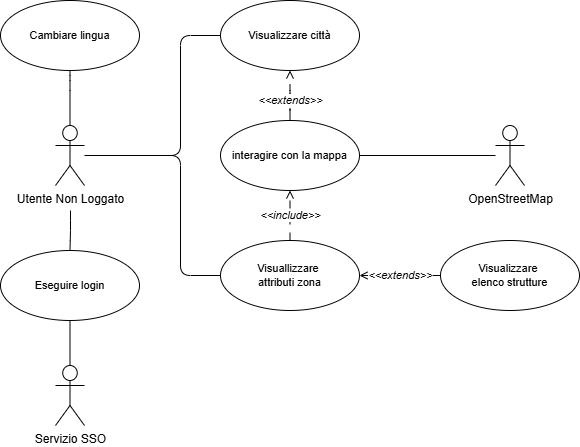
\includegraphics[width=0.8\textwidth]{UseCase_diagrams/NonLoggato.drawio.png}
        \caption{Use Case Diagram dell'Utente non loggato}
    \end{figure}

    \subsection{Visualizzare città}
        \subsubsection{Riassunto}
            Questo Use Case descrive come l'utente può visualizzare gli attributi e la mappa della città
        \subsubsection{Descrizione}
            \begin{itemize}
                \item Il sistema mostra nella parte sinistra dello schermo gli attributi demografici e riguardanti la soddisfazione della città
                \item Il sistema mostra nella parte destra dello schermo la mappa della città suddivisa nella zona selezionata (Estensione 1)
            \end{itemize}
        \subsubsection{Estensioni}
            \begin{itemize}
                \item La tipologia di zona selezionata di default è quella dei quartieri
            \end{itemize}
    
    \subsection{Interagire con la Mappa}
        \subsubsection{Riassunto}
            Questo Use Case descrive come l'utente può interagire con la mappa
        \subsubsection{Descrizione}
            \begin{itemize}
                \item L'utente non loggato posiziona il cursone all'interno dello spazio dedicato alla mappa
                \item Se l'utente utilizza la rotella del mouse oppure uno dei pulsanti presenti in uno degli angoli della mappa
                \item Attraverso le funzionalità fornite da OpenStreetMap la mappa ingrandisce o diminuisce la dimensione dello zoom (Eccezione 1)
                \item Se l'utente preme e trascina il cursore
                \item Attraverso le funzionalità fornite da OpenStreetMap la mappa sposta il focus centrale in funzione del cursore (Eccezione 2)
                \item Se l'utente non loggato seleziona una delle zone all'interno della visuale della mappa (Estensione 1)
                \item Il sistema posiziona il focus centrale della mappa al centro della zona selezionata e ne modifica successivamente lo zoom, il colore e lo spessore dei bordi
                \item Il sistema passa successivamente allo UseCase "Visualizzare zona" della sezione scelta
            \end{itemize}
        \subsubsection{Eccezioni}
            \begin{enumerate}
                \item Nel caso in cui l'utente non loggato cercasse di aumentare o diminuire lo zoom oltre ai limiti imposti, il sistema deve bloccare la nuova modifica allo zoom
                \item Nel caso in cui l'utente non loggato cercasse di spostare il focus centrale oltre ai limiti della città, il sistema deve bloccare la nuova modifica allo spostamento del focus centrale
            \end{enumerate}
        \subsubsection{Estensioni}
            \begin{enumerate}
                \item Nel caso in cui l'utente cliccasse su di una zona già selezionata questa riporterebbe allo UseCase "Visualizzare città"
                \item L'utente, selezionando il pulsante presente nell'angolo della mappa, potrà visualizzare un menù a pop-up e successivamente modificare la tipologia di divisione presente all'interno della mappa
            \end{enumerate}
    
    \subsection{Visualizzare zona}
        \subsubsection{Riassunto}
            Questo Use Case descrive come l'utente può visualizzare la zona selezionata della città
        \subsubsection{Descrizione}
            \begin{enumerate}
                \item Dopo aver interagito con la mappa ed aver selezionato una zona
                \item Il sistema mostra nella parte sinistra dello schermo la mappa centrata sul centro della zona selezionata
                \item Il sistema mostra nella parte destra dello schermo gli attributi demografici e riguardanti la soddisfazione della zona della città selezionata
            \end{enumerate}

    \subsection{Visualizzare elenco strutture}
        \subsubsection{Riassunto}
            Questo Use Case descrive come l'utente può accedere e visualizzare l'elenco delle strutture che forniscono un servizio al cittadino
        \subsubsection{Descrizione}
            \begin{enumerate}
                \item L'utente non loggato preme uno degli attributi presenti a schermo (Eccezione 1)
                \item Il sistema presenta a schermo, ove prima erano presenti gli attributi riguardanti la zona selezionata, una tabella contenente una lista numerata di strutture che offrono il servizio selezionato in precedenza
                \item Il sistema deve successivamente segnalare sulla mappa la posizione delle varie strutture, attraverso un segnalino contenente il numero identificativo presente in tabella della struttura
            \end{enumerate}
        \subsubsection{Eccezioni}
            \begin{enumerate}
                \item Nel caso in cui per una tipologia di dato non fossero presenti strutture il sistema non deve fare nulla
            \end{enumerate}
        \subsubsection{Estensioni}
            \begin{enumerate}
                \item Nel caso in cui l'utente cliccasse il pulante per chiudere la tabella il sistema tornerà alla visualizzazione della zona selezionata in precedenza
            \end{enumerate}

    \subsection{Cambiare lingua}
        \subsubsection{Riassunto}
            Questo Use Case descrive come l'utente può cambiare la lingua dei vari testi presenti nel programma
        \subsubsection{Descrizione}
            \begin{enumerate}
                \item L'utente preme sul menù a tendina presente nella header e seleziona la sezione riguardante la modifica della lingua
                \item Il sistema presenterà a schermo un menù pop-up contenente la lista di lingue per le quali è disponibile la traduzione
                \item Se l'utente seleziona la lingua e clicca il pulsante di conferma (Eccezione 1 e 2)
                \item Il sistema ricarica la pagina selezionata con i testi nella lingua selezionata
            \end{enumerate}
        \subsubsection{Eccezioni}
            \begin{enumerate}
                \item Nel caso in cui l'utente non loggato selezionasse e confermasse la lingua già selezionata, il sistema deve chiudere il pop-up senza apportare alcuna modifica
            \end{enumerate}

    \subsection{Login}
        \subsubsection{Riassunto}
            Questo Use Case descrive come l'utente non loggato può eseguire il login
        \subsubsection{Descrizione}
            \begin{enumerate}
                \item L'utente preme sul menù a tendina presente all'interno della header e seleziona la sezione riguardante il login
                \item Il sistema reindirizza l'utente alla pagina del service provider della provincia di Trento dal quale potrà accedere al login tramite sistema SSO
                \item Il sistema SSO verifica l'identità dell'utente in questione e la ritorna al sistema (Eccezione 1)
                \item Il sistema controlla che per l'identità certificata dal sistema SSO esista un'account collegato (Eccezione 1)
                \item Il sistema assegna dunque un'identità all'utente assegnandogli il ruolo di proprietà
                \item Il sistema successivamente al login sostituisce l'icona del login con l'immagine profilo dell'account al quale si ha fatto l'accesso e reindirizza l'utente allo UseCase "visualizzare città"
            \end{enumerate}
        \subsubsection{Eccezioni}
            \begin{enumerate}
                \item Nel caso in cui l'autenticazione fallisse o non vi fossero account collegati il sistema ritorna alla pagina dalla quale si ha provato a fare il login
            \end{enumerate}


\section{\underline{Utente Sondaggista}}
    Di seguito i requisiti associati all'Utente Sondaggista:
    \begin{itemize}
        \item \textbf{RF6}: Logout
        \item \textbf{RF7}: Visualizzazione dati sondaggisti
        \item \textbf{RF9}: Creazione nuovi sondaggi
        \item \textbf{RF10.1}: Aggiungere voti ai sondaggi
        \item \textbf{RF10.2}: Rimuovere voti ai sondaggi
    \end{itemize}
    \begin{figure}[H]
        \centering
        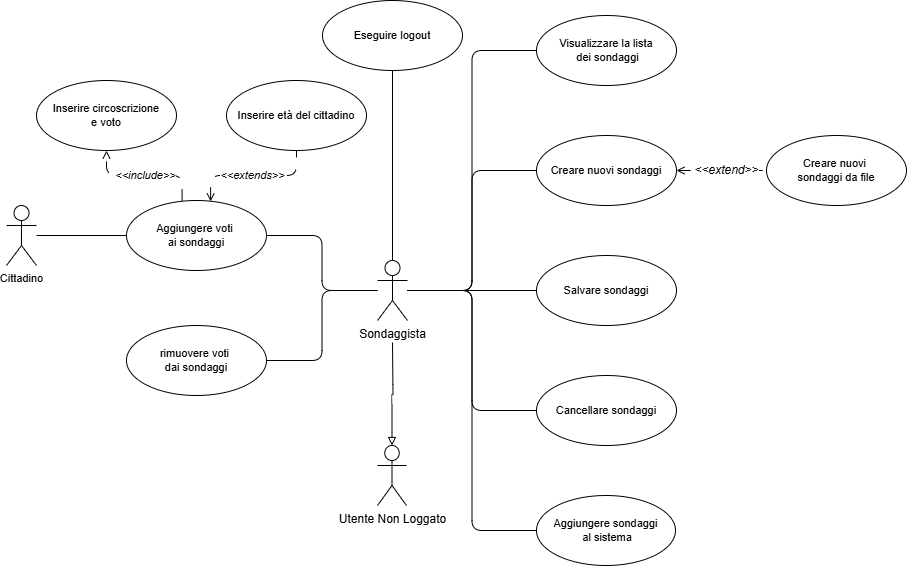
\includegraphics[width=0.8\textwidth]{UseCase_diagrams/Sondaggista.drawio.png}
        \caption{Use Case Diagram dell'Utente sondaggista}
    \end{figure}

    \subsection{Logout}
        \subsubsection{Riassunto}
            Questo Use Case descrive come l'utente può fare logout
        \subsubsection{Descrizione}
            \begin{enumerate}
                \item L'utente sondaggista preme sull'icona contenente l'immagine profilo nella header
                \item Il sistema apre un menù a tendina con la sezione 'Logout'
                \item L'utente preme sulla sezione 'Logout'
                \item Il sistema ricarica la pagina riportando l'utente alla 'visualizzazione città', scollegandolo dall'account sondaggista al quale era collegato e riportando l'utente allo stato di Utente non loggato
            \end{enumerate}
        \subsubsection{Eccezioni}
            \begin{enumerate}
                \item Nel caso in cui fosse aperta il menù a tendina con la sezione logout e venisse successivamente premuto un qualsiasi altro punto sullo schermo il sistema deve chiudere il menù a tendina
            \end{enumerate}

    \subsection{Visualizzazione dati sondaggisti}
        \subsubsection{Titolo}
            Questo Use Case descrive come l'utente sondaggista visualizzerà l'interfaccia per gestire i sondaggi
        \subsubsection{Descrizione}
            \begin{enumerate}
                \item Il sistema mostra nel riquadro in alto a sinistra dello schermo l'interfaccia per la creazione di nuovi sondaggi con relative caselle di testo e pulsante per la creazione
                \item Il sistema mostra nel riquadro in basso a sinistra dello schermo l'interfaccia per il caricamento dei sondaggi attraverso pulsante o "drag and drop"
                \item Il sistema mostra nel riquadro in alto a destra dello schermo l'elenco dei sondaggi non ancora caricati, o in fase di caricamento, a sistema (Eccezione 1)
                \item Il sistema mostra nel riquadro in basso a destra dello schermo l'elenco dei sondaggi già caricati a sistema con relativo stato di accettazione (Eccezione 1)
            \end{enumerate}
        \subsubsection{Eccezioni}
            \begin{enumerate}
                \item Nel caso in cui non fossero presenti sondaggi all'interno di uno degli elenchi il sistema mostrerà a schermo un messaggio per avvisare che tale sezione risulta vuota
            \end{enumerate}
    
    \subsection{Creazione nuovi sondaggi} %to do: da discutere se ha senso fare un activity diagram di ciò, ci sono tanti se e tanti include
        \subsubsection{Titolo}
            Questo Use Case descrive come l'utente sondaggista può aggiungere nuovi sondaggi
        \subsubsection{Descrizione}
            \begin{enumerate}
                \item 
            \end{enumerate}
        \subsubsection{Eccezioni}
        \subsubsection{Estensioni}
    
    \subsection{Aggiungere voti ai sondaggi}
        \subsubsection{Titolo}
            Questo Use Case descrive come l'utente sondaggista può aggiungere nuovi voti ai sondaggi
        \subsubsection{Descrizione}
            \begin{enumerate}
                \item Il sondaggista inserisce la circoscrizione di appartenenza del cittadino (Estensione 1)
                \item Il sistema fornisce l'interfaccia utilie per votare
                \item Il cittadino inserisce il proprio voto e clicca il pulsante di conferma
                \item Il sistema torna all'interfaccia 
            \end{enumerate}
        \subsubsection{Eccezioni}
        \subsubsection{Estensioni}
            \begin{enumerate}
                \item Nel caso in cui il cittadino fosse d'accordo l'utente sondaggista potrà inserire anche la fascia d'età del cittadino 
            \end{enumerate}